\documentclass[12pt]{article}
% Francais UTF8
\usepackage[french]{babel}
\usepackage[utf8]{inputenc}
\usepackage[T1]{fontenc}
\usepackage{lmodern}
\usepackage{graphicx}
\usepackage[small]{caption}
\usepackage{amsmath, amssymb}
\newcommand{\R}{\mathbb{R}}
\newcommand{\Z}{\mathbb{Z}}

\newtheorem{theorem}{Théorème}
\newtheorem{definition}{Définition}

\begin{document}
\author{Gaspard Jankowiak \quad Antoine Levitt\\ Tuteur : Antoine Girard}
\title{Modèles de création d'opinion dans des réseaux sociaux}
\maketitle
\abstract{Bonjour}
\tableofcontents
\newpage


\section{Introduction}
Blabla


\section{Modèles de communautés}
\subsection{Définitions}
Dans toute la suite, $(E, V)$ désigne un graphe à $n$ n\oe uds et $m$
arêtes non orienté : les éléments de $V$ sont des ensembles à deux
éléments de $E$. Ce graphe représente un réseau de $n$ individus, liés
par des relations spécifiques au domaine d'intérêt. Par exemple, on
peut prendre pour $E$ les individus d'un réseau social en ligne (type
Facebook, Myspace ...), et pour $V$ leurs relations d'amitié : $\{i,
j\} \in V$ si et seulement si les individus $i$ et $j$ sont amis. À chaque individu
$i$ on associe une valeur réelle $x_i$ représentant son opinion :
l'état des opinions est donc représenté par un vecteur $x \in
\R^n$. On peut très facilement étendre ce modèle avec des opinions à valeurs
dans $\R^d$.

Tout d'abord, quelques rappels de théorie des graphes. On note $d_i$
le degré du noeud $i$, égal au nombre d'arêtes incidentes au noeud
$i$ : $d_i = card \{v \in V | i \in v\}$. À cette notion est
associée celle de {\bf matrice des degrés} $D$, matrice diagonale
de taille $n \times n$ telle que $D_{i i} = d_i$. On définit
également la {\bf matrice d'incidence} $A$ telle que $A_{i j} = 1$
si $\{i, j\} \in V$, $0$ sinon. Le graphe étant non orienté, cette
matrice est symétrique.

On utilise ces notions pour construire la matrice qui nous sera
utile par la suite, la {\bf matrice Laplacienne}, définie par $L
= D - A$. On a donc $L_{i j} = d_i$ si $i = j$, $L_{i j} = 1$ si
$i$ est adjacent à $j$, et $L_{i j} = 0$ sinon. Son nom vient du
fait que c'est l'analogue pour un graphe quelconque de
l'opérateur Laplacien classique : pour un graphe représentant un
espace à $2$ dimensions discrétisé, c'est-à-dire dont les noeuds
sont les points $(i \Delta x, j \Delta y)$, on a $L(x) (i, j) =
4 x(i, j) - x(i+1, j) - x(i-1, j) - x(i, j+1) - x(i, j-1)$, et
on retrouve au signe près le Laplacien discrétisé. Les
propriétés (notamment spectrales) de cette matrice renseignent
sur le graphe, et c'est cette approche que l'on va utiliser dans
notre étude.

\subsection{Graphes utilisés}
On utilise principalement deux graphes, représentés figure
\ref{graphes}.  Le premier est le réseau d'amitié dans un club de
karaté d'une université américaine dans les années 70, contenant 34
membres \cite{zachary}. Le second est le graphe d'interactions d'une
communauté de 62 dauphins \cite{dolphins}.

\begin{figure}[htb]
  \centering
  (a)
  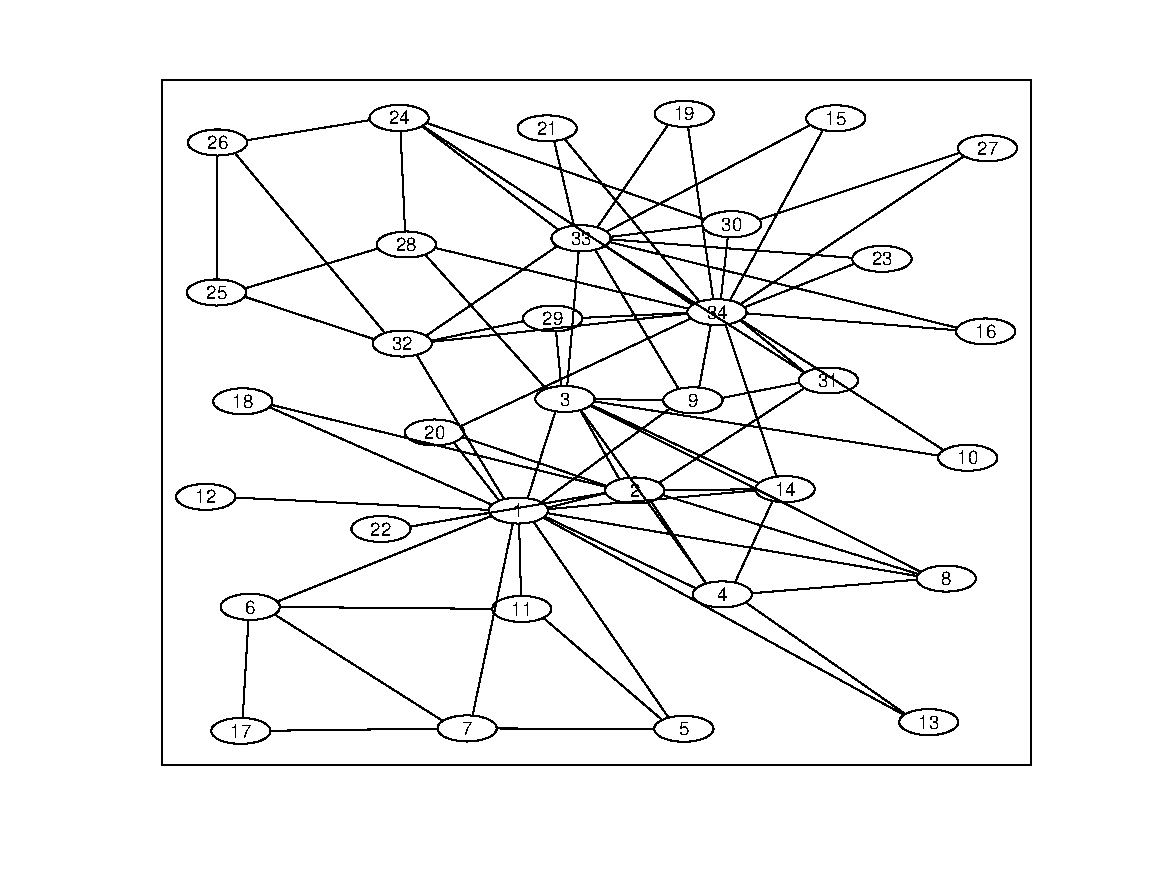
\includegraphics[width=.4 \textwidth]{zachary}
  (b)
  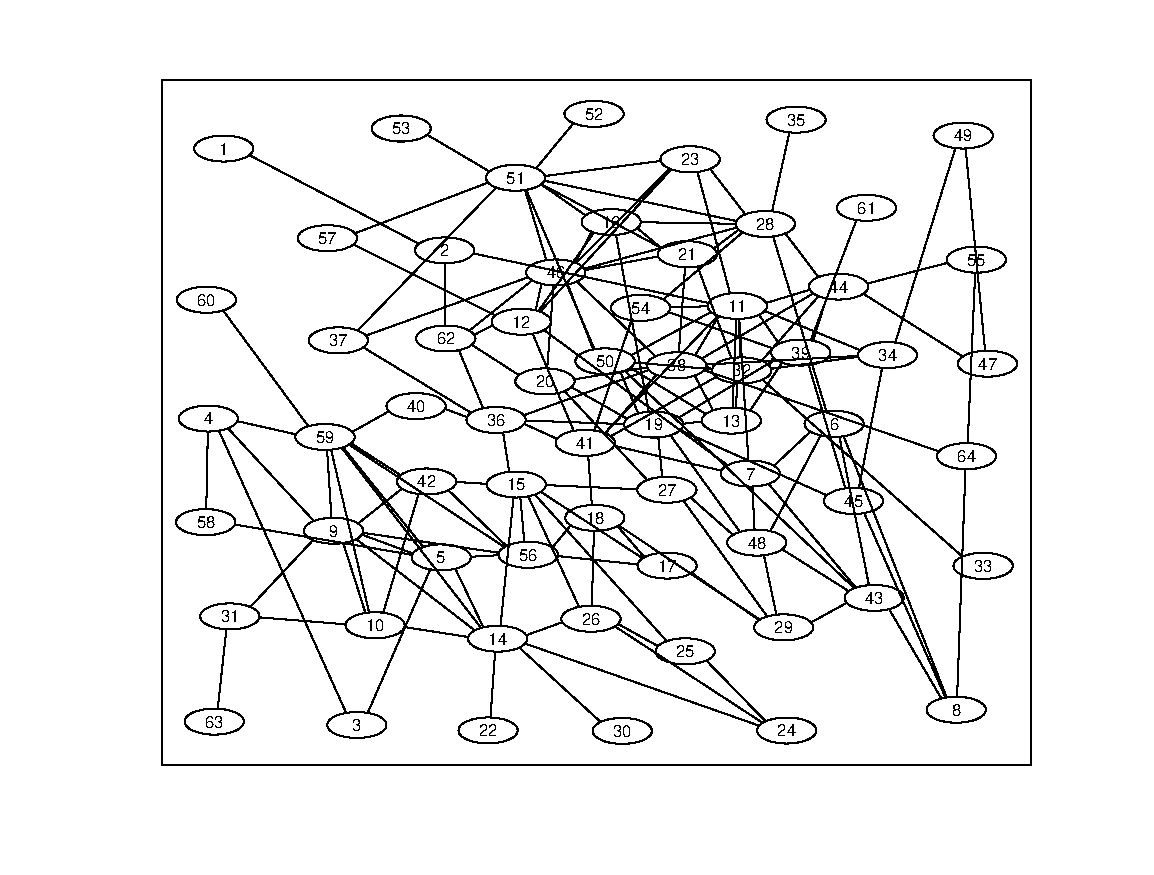
\includegraphics[width=.4 \textwidth]{dolphins}
  \caption{Club de karaté de Zachary (a), et communauté de dauphins (b).}
  \label{graphes}
\end{figure}

Ces graphes ont été choisis parce qu'ils possèdent des
structures de communauté qu'on peut mettre en évidence plus
facilement que sur un graphe aléatoire. Sur la communauté de
dauphins, il a été observé une partition des dauphins au départ
de l'un d'entre eux, ce qui fournit une base expérimentale à
notre étude.

\subsection{Modèles de création de consensus}
Étant donné un vecteur d'opinions initiales $x^0$, on
s'intéresse à l'évolution de ces opinions dans différents
modèles. Le modèle de base est l'équation différentielle
\begin{equation}
  \label{eq_diff}
  \dot x + L x = 0.
\end{equation}

On peut interpréter cette équation en la réécrivant sous forme scalaire :
\begin{equation}
  \label{eq_diff_scal}
  \dot {x}_i = \sum_{j \in N_i} (x_j - x_i),
\end{equation}
où $N_i$ est le voisinage de $i$, c'est à dire tous les noeuds
qui lui sont adjacents. Chaque personne révise son opinion en
fonction de celle de ses voisins. Intuitivement, on s'attend à
ce que ce modèle provoque une convergence vers un
consensus. Cette intuition est corroborée par la ressemblance de
(\ref{eq_diff}) avec l'équation de la chaleur, dont les
propriétés de convergence vers la valeur moyenne sont bien
connues. En fait, dans le cas d'un graphe représentant un espace
discrétisé, (\ref{eq_diff}) est tout simplement la
discrétisation par différences finies de l'équation de la
chaleur.

\subsection{Propriétés spectrales de $L$}
\section{Analyse spectrale de graphes et partitionnement}

\begin{thebibliography}{2}
\bibitem{zachary} W. W. Zachary, An information flow model for conflict and fission in small groups, Journal of Anthropological Research 33, 452-473 (1977)
\bibitem{dolphins} D. Lusseau, K. Schneider, O. J. Boisseau, P. Haase, E. Slooten, and S. M. Dawson, Behavioral Ecology and Sociobiology 54, 396-405 (2003)
\end{thebibliography}
\end{document}
